\documentclass[9pt]{extarticle}

\usepackage{amsmath}
\usepackage{multicol}
\usepackage{titlesec}
\usepackage{enumitem}
\usepackage{adjustbox}
\usepackage{stmaryrd}
\usepackage{tikz}
\usepackage{graphicx}
\usetikzlibrary{shapes, positioning}
\setlist{nosep}
\titleformat{\subsection}[runin]{\normalfont\Large\bfseries}{\thesubsection.}{6pt}{}[]
\titlespacing*{\subsection}{0pt}{0pt}{0pt}



% Disable warnings
% chktex-file 1

\usepackage[margin=0.35in, portrait]{geometry} % may exceed print margins
\pagestyle{empty}

\usepackage[dvipsnames]{xcolor}

% Colour-blind friendly scheme
\definecolor{MyMagenta}{rgb}{0.91,0.16,0.54}
\definecolor{MyGreen}{rgb}{0.4,0.65,0.12}
\definecolor{MyPurple}{rgb}{0.46,0.44,0.7}
\definecolor{MyOrange}{rgb}{0.85,0.37,0.01}
\definecolor{MyEmerald}{rgb}{0.11,0.62,0.47}
\definecolor{MyYellow}{RGB}{230,171,2}
\definecolor{MyBlue}{RGB}{0,114,178}

\colorlet{defc}{MyMagenta}
\colorlet{lemc}{MyGreen}
\colorlet{corc}{MyPurple}
\colorlet{propc}{MyOrange}
\colorlet{thmc}{MyEmerald}
\colorlet{alg}{MyYellow}
\colorlet{ex}{MyBlue}

\colorlet{namec}{DarkOrchid}

\newcommand{\wde}[1]{\textcolor{defc}{\newline\textbf{DEF}} (\textcolor{namec}{\textit{#1}})}
\newcommand{\wl}[1]{\textcolor{lemc}{\newline\textbf{LEM}} (\textcolor{namec}{\textit{#1}})}
\newcommand{\wc}[1]{\textcolor{corc}{\newline\textbf{COR}} (\textcolor{namec}{\textit{#1}})}
\newcommand{\wpr}[1]{\textcolor{propc}{\newline\textbf{PROP}} (\textcolor{namec}{\textit{#1}})}
\newcommand{\wt}[1]{\textcolor{thmc}{\newline\textbf{THM}} (\textcolor{namec}{\textit{#1}})}
\newcommand{\wa}[1]{\textcolor{alg}{\newline\textbf{ALG}} (\textcolor{namec}{\textit{#1}})}
\newcommand{\wpf}[1]{\textcolor{red}{\newline\textit{#1}}}  % Proof
\newcommand{\we}[1]{\textcolor{ex}{\newline\textbf{EX}} (\textcolor{namec}{\textit{#1}})}

\usepackage{amsmath}
\usepackage{amsthm}
\usepackage{amssymb}
\usepackage{tipa}
\usepackage{algpseudocode}
\usepackage{amssymb}
\usepackage{ebproof}

% \fontsize{2}

\begin{document}
  \begin{multicols}{2}
  \subsection*{Secure Development}
  \wde{CVE Format and Meaning}{
    Common Vulnerabilities and Exposures (CVE) is a list of publicly disclosed cybersecurity vulnerabilities and exposures. Each CVE entry includes:
    \begin{itemize}
        \item CVE ID: a unique identifier for the vulnerability.
        \item Description: a brief summary of the vulnerability.
        \item References: links to advisories or reports that provide more details.
    \end{itemize}
}

\wde{CVSS - Common Vulnerability Scoring System}{
    The Common Vulnerability Scoring System (CVSS) is a standard for assessing the severity of software vulnerabilities. It provides a numerical score based on the following metrics:
    \begin{itemize}
        \item \textbf{Base Metrics}: Characteristics of the vulnerability itself.
        \item \textbf{Temporal Metrics}: Characteristics that change over time (e.g., exploit availability).
        \item \textbf{Environmental Metrics}: Characteristics specific to the organization's environment.
    \end{itemize}
    The CVSS score helps organizations prioritize and respond to vulnerabilities based on their severity.
}
\wde{CVSS Base Metrics}{
    The CVSS Base Metrics include:
    \begin{itemize}
        \item \textbf{Attack Vector}: How the vulnerability is exploited \textit{(Local, Adjacent, Network)}.
        \item \textbf{Attack Complexity}: The level of expertise required to exploit the vulnerability \textit{(Low, High)}.
        \item \textbf{Privileges Required}: The level of privileges an attacker needs to exploit the vulnerability \textit{(None, Low, High)}.
        \item \textbf{User Interaction}: Whether user interaction is required to exploit the vulnerability \textit{(None, Required)}.
        \item \textbf{Scope}: Whether the vulnerability impacts the vulnerable component only or can affect other components \textit{(Unchanged, Changed)}.
        \item \textbf{Confidentiality, Integrity, Availability Impact}: The impact on the security properties of confidentiality, integrity, and availability \textit{(None, Low, High)}.
    \end{itemize}
}
\wde{Common Weakness Enumeration (CWE)}{
    The CWE is a community-developed list of common software security weaknesses. It provides a classification of software vulnerabilities to help developers understand and mitigate risks.
}
\wde{Security Properties}{
    Key security properties that must be considered in secure programming include:
    \begin{enumerate}
        \item \textbf{Confidentiality}: Data is only available to the people intended to access it.
        \item \textbf{Integrity}: Data and system resources are only changed in appropriate ways by appropriate people.
        \item \textbf{Availability}: Systems are ready when needed and perform acceptably.
        \item \textbf{Authentication}: The identity of users is established (or you're willing to accept anonymous users).
        \item \textbf{Authorization}: Users are explicitly allowed or denied access to resources.
        \item \textbf{Nonrepudiation}: Users can't perform an action and later deny performing it.
    \end{enumerate}
}

\wde{STRIDE}{
    STRIDE is a mnemonic for categories of security threats, along with the corresponding security properties that each threat type attacks:
    \begin{itemize}
        \item \textbf{Spoofing}: Attacker pretends to be someone else. \textit{(Attacks Authentication)}
        \item \textbf{Tampering}: Attacker alters data or settings. \textit{(Attacks Integrity)}
        \item \textbf{Repudiation}: User can deny making an attack. \textit{(Attacks Non-repudiation)}
        \item \textbf{Information Disclosure}: Loss of personal information. \textit{(Attacks Confidentiality)}
        \item \textbf{Denial of Service}: Preventing proper site operation. \textit{(Attacks Availability)}
        \item \textbf{Elevation of Privilege}: User gains higher privileges. \textit{(Attacks Authorization)}
    \end{itemize}
}


\wde{Saltzer's Classic Principles}{
    Saltzer and Schroeder's principles provide guidelines for secure design:
    \begin{enumerate}
        \item \textbf{Economy of Mechanism}: Keep the design simple.
        \item \textbf{Fail-Safe Defaults}: Default to secure configurations; fail closed with no single point of failure.
        \item \textbf{Complete Mediation}: Check permissions on every access; ensure that all access requests are verified.
        \item \textbf{Open Design}: Assume that attackers have access to the source code and specifications; design should not rely on obscurity.
        \item \textbf{Separation of Privilege}: Require multiple conditions to grant access to sensitive operations; don’t permit an operation based on a single condition.
        \item \textbf{Least Privilege}: Grant only the minimum privileges necessary for users or processes; no more privileges than what is needed.
        \item \textbf{Least Common Mechanism}: Minimize shared resources; be cautious of mechanisms that are shared among users.
        \item \textbf{Psychological Acceptability}: Ensure that security measures are user-friendly and do not hinder usability; security should be intuitive for users.
    \end{enumerate}
}


\wde{McGraw's Three Pillars}{
    McGraw's approach is built on three pillars:
    \begin{enumerate}
        \item \textbf{Applied Risk Management}: Identify, rank, and track risks using threat modeling to uncover security risks.
        \item \textbf{Software Security Touchpoints}: Integrate security-related activities throughout the software development lifecycle.
        \item \textbf{Knowledge}: Leverage existing knowledge, programming guidelines, and known exploits to enhance security practices.
    \end{enumerate}
}

\wde{McGraw's Seven Touchpoints}{
    McGraw identified 7 touchpoints that could be integrated in the traditional software development lifecycle (SDLC)
    \begin{enumerate}
        \item \textbf{Abuse Cases}: Identify potential misuse scenarios.
            \begin{itemize}
                \item Artifacts: Use case documents, threat models.
                \item Problems: Failure to consider all misuse scenarios can lead to unaddressed vulnerabilities.
                \item Bad Example: Ignoring input validation in a web application leading to SQL injection.
            \end{itemize}
        \item \textbf{Security Requirements}: Define security needs early in the process.
            \begin{itemize}
                \item Artifacts: Security requirement specifications, risk assessment reports.
                \item Problems: Vague or incomplete security requirements can result in inadequate protection.
                \item Bad Example: A requirement stating "the application should be secure" without specifics on encryption or access controls.
            \end{itemize}
        \item \textbf{Architectural Risk Analysis}: Assess risks in design and architecture.
            \begin{itemize}
                \item Artifacts: Architecture diagrams, risk analysis documents, design specifications.
                \item Problems: Failing to identify security flaws in the architecture can lead to critical vulnerabilities.
                \item Bad Example: Designing a system without considering the security of third-party components.
            \end{itemize}
        \item \textbf{Risk-Based Security Testing}: Focus on testing based on risk analysis.
            \begin{itemize}
                \item Artifacts: Test plans, test cases, risk assessment matrices.
                \item Problems: Inadequate testing of high-risk areas may leave critical vulnerabilities untested.
                \item Bad Example: Conducting extensive tests on low-risk features while neglecting authentication mechanisms.
            \end{itemize}
        \item \textbf{Code Review}: Inspect code for security vulnerabilities.
            \begin{itemize}
                \item Artifacts: Source code, code review checklists, static analysis reports.
                \item Problems: Insufficient or poorly structured code reviews can miss significant vulnerabilities.
                \item Bad Example: Relying solely on automated tools without manual review, leading to overlooked security issues.
            \end{itemize}
        \item \textbf{Penetration Testing}: Test the system for vulnerabilities in a real-world context.
            \begin{itemize}
                \item Artifacts: Penetration testing reports, vulnerability assessment tools, exploitation scripts.
                \item Problems: Conducting penetration tests without understanding the system can result in incomplete assessments.
                \item Bad Example: External testers not familiar with the application’s architecture, leading to ineffective testing.
            \end{itemize}
        \item \textbf{Security Operations}: Manage security during the deployment phase.
            \begin{itemize}
                \item Artifacts: Security operation procedures, incident response plans, monitoring logs.
                \item Problems: Lack of continuous monitoring can lead to undetected security incidents.
                \item Bad Example: Deploying an application without proper logging and monitoring, making incident response difficult.
            \end{itemize}
    \end{enumerate}
}

\wt{Dijkstra's Observation on Testing}{
    Dijkstra's famous remark states:
    \begin{quote}
        "Testing shows the presence, not the absence of bugs."
    \end{quote}
    This highlights the importance of comprehensive testing strategies and the understanding that passing tests do not guarantee that no bugs exist in the software.
}

\wde{Building Security In Maturity Model (BSIMM)}{
It is a blueprint/software security framework for following good practices of software development. It is data-driven and so the practices are collated by examining the strategies that companies are utilising to produce secure software.
% BSIMM consists of a total of 126 activities that are assigned maturity levels (1-3), where level 1 indicates the most mature practices that are commonly adopted by companies. 
The framework is composed of four domains: 
Governance, Intelligence, SSDL Touchpoints, and Deployment, with each domain containing three practices (for a total of 12 practices).
\begin{itemize}
    \item Governance: Establishing security policies and practices.
    \begin{itemize}
        \item Strategy and metrics
        \item Compliance and policy.
        \item Training.
    \end{itemize}
    \item Intelligence: Gathering security metrics and threat intelligence.
    \begin{itemize}
        \item Attack models.
        \item Security features.
        \item Standards and requirements.
    \end{itemize}
    \item Development: Integrating security into the development process.
    \begin{itemize}
        \item Code review.
        \item Security testing.
        \item Architecture analysis.
    \end{itemize}
    \item Deployment: Ensuring secure deployment and operations.
    \begin{itemize}
        \item Environment hardening.
        \item Software environment.
        \item Incident management.
    \end{itemize}
\end{itemize}
}



  \subsection*{Programming Errors}
  \wde{Memory Safety}{
    A programming language or analysis tool is said to enforce memory safety if it 
    ensures that reads and writes stay within clearly defined memory areas,
    belonging to different parts of the program.
    Memory areas are often delineated with types and a typing discipline.
}
\wde{Type Safety}{
    A programming language, analysis tool or runtime is said to enforce type safety if it 
    has a clearly specified typing discipline for data values and it ensures that 
    data values (representations) for types stay within the domain of those types during 
    program execution.
}

\wt{Type Safety implies Memory Safety}{
    Type safety implies memory safety (provided it does bounds checking).
    Converse \textbf{not} true.
}
\wde{Buffer Overflow}{
    Buffer overflows arise when a region of memory exceeds its allocated size, resulting in the overwriting of adjacent memory that may be used elsewhere in the program. This can lead to unexpected behavior in the program's execution.
    A buffer overflow exploits the stack layout to typically overwrite the return address of a function to 
    perform arbitrary code execution (shellcode or return-to-libc).
    This attacks the integrity of the program and can lead to privilege escalation.
    It's also possible to attack the availability of the program by causing a denial of service - by crashing the program.
}

\wde{Out-by-one/Arithmetic Errors}{
    Can lead to buffer overflows, memory corruption, and other security vulnerabilities.
}

\wde{Faulty/Missing Error Condition Checking}{
    Not checking for error conditions can lead to unexpected behavior and security vulnerabilities.
}

\wde{Format String Vulnerabilities}{
    Can lead to memory corruption, arbitrary code execution, and other security vulnerabilities.
    In C and C++, the \texttt{printf} function is vulnerable to format string attacks if the format string is user-controlled.
}
\wde{Stack Layout}{
    \begin{center}
        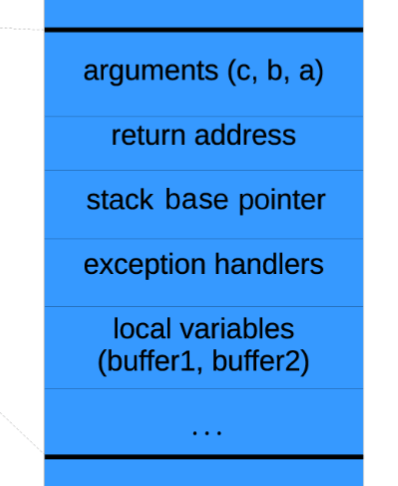
\includegraphics[width=0.5\linewidth]{images/stack-layout.png}
    \end{center}
The above diagram shows the layout of the stack in memory. The stack grows downwards, with the stack pointer pointing to the top of the stack. The stack frame contains the return address, arguments, local variables, and saved registers. The frame pointer points to the base of the current stack frame (current function).
}

  \subsection*{Platform and Operating System Level Attacks}
  \wde{Assembly Programs and Shell-Code Attacks}{
    Assembly programs can be used to create shellcode which is injected into vulnerable applications through buffer overflows. 
    Could spawn a shell (arbitrary code execution), reverse shell (remote code execution), or other malicious activities.
}
\wde{OS Command Injection/Environment Variables}{
    It's important to be careful with programs that use environment variables to execute commands.
    In particular \texttt{PATH} and \texttt{LD\_LIBRARY\_PATH} can be manipulated to execute arbitrary
    code. 
}

\wde{Unix File Permission Codes}{
    Unix file permissions are represented by a 10 character string. The first character is the file type, the next three are the owner's permissions, the next three are the group's permissions, and the last three are the world's permissions (everyone else). The permissions can be:
    \begin{itemize}
        \item \texttt{r} - read (4)
        \item \texttt{w} - write (2)
        \item \texttt{x} - execute (1)
    \end{itemize}
    Common file types are:
    \begin{itemize}
        \item \texttt{-} - regular file
        \item \texttt{d} - directory
        \item \texttt{l} - symbolic link
    \end{itemize}
}
\wde{Permission Attacks}{
    Exploring the file system and looking for files with weak permissions can be a good way to find vulnerabilities.
}

\wde{Stack Canary / StackGuard}{
    A form of \textbf{Tamper Detection} that can be used to detect buffer overflows.
    StackGuard canaries prevent buffer overflow attacks by inserting random values near the return pointer and checking their integrity before returning.
    While effective against return pointer overwriting, they don't protect against modifying local variables or preventing Denial of Service attacks that intentionally trigger canary detection.
    Also not effective against return-to-libc (ret2libc) or return-oriented programming (ROP) attacks.
}
\wde{Control-Flow Integrity (CFI)}{
    A more powerful defense mechanism that ensures the code execution follows a pre-defined control graph.
    This \textit{could} prevent return-to-libc and ROP attacks.
}

\wde{Seperation Mechanisms}{
    \begin{itemize}
        \item Hardware Memory Protection 
        \begin{itemize}
            \item Memory Fences: These seperate memory accesses between OS and user code, providing one-way protection 
            \item Base and Bounds Registers: Enforce seperation between programs by controlling access to specific memory ranges, thus preventing unauthorized memory access
            \item Tagged Architecture: Assign tags to memory locations that dictate access rights (read,write,execute), although not widely used in modern systems
        \end{itemize}
        \item Paging splits programs/data into pieces.
        \begin{itemize}
            \item Data Execution Prevention (DEP) / Write XOR Execute (W\^{}X): Prevents code from executing in data regions (making injected shellcode non-executable)
        \end{itemize}
        \item Process Isolation (EXTRA)
        \begin{itemize}
            \item Virtual Memory: Each process operates in its own virtual address space, preventing unauthorized access to other processes
            \item Containerisation: Isolates processes in containers, preventing unauthorized access to other processes. Reduces the attack surface area 
            and worst-case it will only compromise the container
        \end{itemize}
    \end{itemize}
}


\wde{Diversification}{
    Make many versions of same program; thwarting attacks that rely on knowing the exact layout of the program in memory.
    \textbf{Address Space Layout Randomization (ASLR)} is a common technique that randomizes the memory layout of a program.
    Could still be suspectible to a brute-force attack of guessing the memory layout.
}


  \subsection*{SQL Injection}
  \wde{Injection}{
    Succinctly defined as part of CWE-74: Improper Neutralization of Special Elements in Output Used by a Downstream Component, i.e. 
    \begin{quote}
    ALWAYS CHECK YOUR INPUTS
    \end{quote}
}

\wde{Metadata}{
    Metadata accompanies the main data and represents additional information about it, such as how to display textual strings or where a string ends. In the context of SQL injection, metadata can influence how queries are constructed and processed.
}

\wde{In-band Representation}{
    In-band representation embeds metadata into the data stream itself, such as using special characters within SQL queries. This can lead to injection vulnerabilities if user input is not properly sanitized.
}

\wde{Out-of-band Representation}{
    Out-of-band representation separates metadata from data, making it less susceptible to injection attacks. For example, using prepared statements allows the SQL engine to distinguish between data and commands.
}

\wde{Input Validation}{
    Input validation can be achieved through blacklisting and whitelisting:
    \begin{itemize}
        \item \textbf{Blacklisting}: Keeping a list of forbidden characters or patterns and rejecting inputs that contain them.
        \item \textbf{Whitelisting}: Keeping a list of allowed characters or patterns and rejecting inputs that do not match.
    \end{itemize}
}

\wde{SQL Injection}{
    SQL Injection (CWE-89) is a command injection (CWE-77) that allows attackers to execute arbitrary SQL queries through user input. This can lead to unauthorized access to the database, data leakage, and data corruption.
}

\wde{Common SQL Injection Techniques}{
    SQL injection techniques can be classified into several categories:
    \begin{itemize}
        \item \textbf{Tautologies}: Injecting code that always evaluates to true.
        \item \textbf{Illegal/Incorrect Queries}: Causing run-time errors to learn information from error messages.
        \item \textbf{Union Queries}: Combining results from multiple queries to extract additional data.
        \item \textbf{Piggy-Backed Queries}: Executing multiple queries in a single request.
        \item \textbf{Inference Pairs}: Using differences in responses to infer information.
        \item \textbf{Stored Procedures}: Exploiting vulnerabilities in stored procedures to execute arbitrary SQL commands.
    \end{itemize}
}

\wde{Prevention and Detection}{
    To prevent SQL injection vulnerabilities, developers can:
    \begin{itemize}
        \item Use prepared statements and parameterized queries.
        \item Implement rigorous input validation and sanitization.
        \item Employ web application firewalls (WAFs) to filter malicious requests.
        \item Regularly test and audit code for vulnerabilities.
    \end{itemize}
}


  \subsection*{Web Application Attacks and Defenses}
  \wde{OWASP - Open Web Application Security Project}{
    The Open Web Application Security Project (OWASP) is a non-profit organization dedicated to improving web application security.
}
\wde{HTTP and Attacks}{
    HTTP (Hypertext Transfer Protocol) is the foundational protocol for data communication on the web. It is stateless, meaning each request from a client to server is treated as an independent transaction. This statelessness can lead to vulnerabilities if not managed properly.
    
    Common attacks on HTTP include:
    \begin{itemize}
        \item \textbf{Session Stealing}: Attackers can hijack a user's session by obtaining their session ID, often through Cross-Site Scripting (XSS) or Cross-Site Request Forgery (CSRF).
        \item \textbf{Authentication Errors}: Flaws in authentication mechanisms can allow unauthorized users to gain access to sensitive information or functionalities.
        \item \textbf{URL Format Attacks}: Manipulating URLs to exploit vulnerabilities in how web applications process parameters.
    \end{itemize}
}

\wde{Session Stealing}{
    Session stealing occurs when an attacker obtains a user's session ID, allowing them to impersonate the user. This can happen through various means, such as:
    \begin{itemize}
        \item \textbf{Cross-Site Scripting (XSS)}: Injecting malicious scripts into web pages to steal session cookies.
        \item \textbf{Cross-Site Request Forgery (CSRF)}: Forcing users to perform actions without their consent.
    \end{itemize}
}

\wde{URL Format Attacks}{
    URL format attacks exploit flaws in how web applications process URLs. Common vulnerabilities include:
    \begin{itemize}
        \item \textbf{Open Redirects}: Allowing attackers to redirect users to malicious sites.
    \end{itemize}
}

\wde{Object References}{
Exploitting XML External Entities (XXE) vulnerabilities allows attackers to read local files, perform remote requests, and execute arbitrary code. 
To prevent XXE attacks, use more restrictive and specific formats for exchanging data, take care with deserialization, configure DTD and XML processors to validate documents, enable security checks, and prevent external entity processing.
}

\wde{Cross-Site Scripting (XSS)}{
    Cross-Site Scripting (XSS) attacks allow attackers to inject malicious scripts into web pages viewed by other users. There are two main types:
    \begin{itemize}
        \item \textbf{Stored XSS}: The malicious script is stored on the server and delivered to users when they access the affected page.
        \item \textbf{Reflected XSS}: The script is reflected off a web server, typically via a URL or form submission.
    \end{itemize}
    
    To mitigate XSS attacks, developers should implement output encoding, input validation, and Content Security Policies (CSP).
}

\wde{Cross-Site Request Forgery (CSRF)}{
    Cross-Site Request Forgery (CSRF) is an attack that tricks a user into executing unwanted actions on a different site where they are authenticated. This can lead to unauthorized transactions or actions. To prevent CSRF attacks:
    \begin{itemize}
        \item Use anti-CSRF tokens in forms.
        \item Implement SameSite cookie attributes.
        \item Validate the Referer header to ensure requests come from trusted sources.
        \item A ``double submit cookie'' approach can also be used where a cookie value is sent in both a cookie and a request parameter and if they don't match, the request is rejected.
    \end{itemize}
}


  \subsection*{Other Application Attacks}
  
\we{
    xz-utils
}{
    The xz-utils vulnerability exploited IFUNCs in the library, allowing runtime function implementation selection.
    Attacker Jia Tan crafted a bash script using M4 macros that manipulated test files and modified the Makefile, creating a binary backdoor.
    The backdoor's IFUNC resolver altered the Global Offset Table, redirecting the `RSA\_public\_decrypt()` function to malicious code.
    When services like SSHD used the library, this enabled arbitrary code execution, demonstrating the risks of dynamic function resolution in shared libraries.
}

\we{Heartbleed}{
    Heartbleed is a serious vulnerability in the OpenSSL cryptographic software library, discovered in 2014. 
    \begin{itemize}
        \item **Failure of Protocol Design**: The flaw allowed attackers to exploit the heartbeat extension of the TLS/DTLS protocols.
        \item **Session Prolongation**: Attackers could prolong sessions without detection, leading to potential data leakage.
        \item **Untrusted Clients**: Clients are inherently untrusted, and the vulnerability allowed them to read sensitive memory from the server.
        \item **Data Leakage Attack**: This resulted in the exposure of private keys, usernames, passwords, and other sensitive data.
    \end{itemize}
}

\we{Shellshock}{
    Shellshock is a vulnerability in the Unix Bash shell that was discovered in 2014, allowing attackers to execute arbitrary commands via environment variables.
    \begin{itemize}
        \item **Bash Attack**: The vulnerability exploited the way Bash handles function definitions, enabling command injection.
        \item **Common in Embedded Systems**: Shellshock is particularly dangerous because shell interpreters are widely used in embedded systems and IoT devices.
        \item **Influence of Environment Variables**: Attackers could manipulate environment variables to execute commands on vulnerable systems.
        \item **Arbitrary Command Execution**: This led to widespread exploitation, allowing attackers to gain unauthorized access and control over affected systems.
    \end{itemize}
}

\we{Spectre and Meltdown}{
    Spectre and Meltdown are vulnerabilities discovered in modern CPUs, affecting nearly all processors manufactured since the late 1990s.
    \begin{itemize}
        \item **Rediscovered Vulnerabilities**: These vulnerabilities exploit speculative execution, a performance optimization technique used in CPUs.
        \item **CPU Speculation**: Attackers could trick the CPU into executing instructions that should not have been run, allowing them to access sensitive data.
        \item **Impact on Web Browsers**: Web browsers with Just-In-Time (JIT) compilation were particularly affected, as they could inadvertently expose data from other processes.
        \item **Isolation Circumvention**: Isolation is a primary defense mechanism that was circumvented, leading to potential data breaches across different applications running on the same hardware.
    \end{itemize}
}

\we{Mirai}{
    Mirai is a malware strain that targets Internet of Things (IoT) devices, discovered in 2016, and is known for launching large-scale DDoS attacks.
    \begin{itemize}
        \item **IoT Device Vulnerabilities**: The malware exploits weak security credentials (default usernames and passwords) in IoT devices.
        \item **DDoS Botnet Army**: Mirai created a botnet army by infecting thousands of IoT devices, which were then used to launch Distributed Denial of Service (DDoS) attacks.
        \item **Cyberattack on Dyn**: The most notable attack was on Dyn, a DNS provider, which disrupted major websites and services, showcasing the vulnerabilities of IoT devices and the potential for large-scale cyberattacks.
    \end{itemize}
}

  \subsubsection*{Advanced Secure Programming}
  \wde{Information Leakage}{
    Information leakage occurs when sensitive data is unintentionally exposed to unauthorized parties. This can happen through various channels, including:
    \begin{itemize}
        \item \textbf{Web Applications}: Poorly configured applications may expose data through error messages or logs.
        \item \textbf{APIs}: APIs that return excessive data or lack proper access controls can leak sensitive information.
        \item \textbf{Session Management}: Insecure session management can allow attackers to steal session IDs and access confidential data.
    \end{itemize}
}

\wde{Race Conditions}{
    Race conditions arise in concurrent systems when multiple processes or threads access shared resources without proper synchronization. This can lead to unexpected behavior, data corruption, or security vulnerabilities:
    \begin{itemize}
        \item \textbf{Time-of-Check to Time-of-Use (TOCTOU)}: A specific race condition where the state of a resource changes between the check and the use, potentially allowing unauthorized access.
        \item \textbf{Data Races}: Occur when two or more threads access shared data simultaneously, and at least one of the accesses is a write.
    \end{itemize}
    They can be prevented by using synchronization mechanisms such as locks, semaphores, or atomic operations. 
}

\wde{Taint Access Control}{
    Taint access control is a security mechanism that tracks the flow of potentially harmful data through a program. The key concepts include:
    \begin{itemize}
        \item \textbf{Tainted Data}: Data that originates from untrusted sources, such as user input.
        \item \textbf{Untainted Data}: Data that is considered safe to use and has been verified.
        \item \textbf{Propagation of Labels}: As data flows through the program, labels indicating whether data is tainted or untainted are propagated, allowing for checks before sensitive operations.
    \end{itemize}
    This approach helps prevent vulnerabilities related to information leakage and ensures that sensitive operations are only performed on trusted data.
    This lets you know \textbf{when} information is leaked, rather than preventing it. 
    Additionally, it only captures direct flows of information, not indirect ones (would be intractable otherwise) therefore it may gloss over some information leaks.
}

\wt{Typability implies No Insecure Flaws}{
    If an output expression has type \textbf{low}, then it cannot be affected by any input of type \textbf{high}. Hence 
    there can be no insecure information flows in the program.
}

% \begin{itemize}
%     \item 
%     \begin{multicols}{2}
%         \begin{prooftree}
%             \hypo{[\textcolor{red}{high}] \vdash C}
%             \infer1{[\textcolor{blue}{low}] \vdash C}
%         \end{prooftree}
            
%         \begin{prooftree}
%             \hypo{[pc] \vdash C_1}
%             \hypo{[pc] \vdash C_2}
%             \infer2{[pc] \vdash C_1; C_2}
%         \end{prooftree}
%     \end{multicols}
%     \item
%     \begin{multicols}{2}
%         \begin{prooftree}
%             \hypo{exp:pc}
%             \hypo{[pc] \vdash C_1}
%             \hypo{[pc] \vdash C_2}
%             \infer3{[pc] \vdash \text{if exp then } C_1 \text{ else } C_2}
%         \end{prooftree}
        
%         \,\,\,
%         \begin{prooftree}
%             \hypo{exp:pc}
%             \hypo{[pc] \vdash C}
%             \infer2{[pc] \vdash \text{while exp do } C}
%         \end{prooftree}
%     \end{multicols}
% \end{itemize}
% }
\wde{Program Analysis Tools for Security}{
    Program analysis tools help identify vulnerabilities in code by analyzing source code or binaries. They can be categorized into two main types:
    \begin{itemize}
        \item \textbf{Static Analysis Tools}: Analyze code without executing it, looking for potential vulnerabilities, coding standards violations, and logic errors. Examples include FindBugs, PMD, and Coverity.
        \item \textbf{Dynamic Analysis Tools}: Analyze code during execution, monitoring runtime behavior to detect issues such as memory leaks, race conditions, and security vulnerabilities. Examples include Valgrind and AddressSanitizer.
    \end{itemize}
}

\wde{Static versus Dynamic Analysis}{
    Both static and dynamic analysis have their strengths and weaknesses:
    \begin{itemize}
        \item \textbf{Static Analysis}:
            \begin{itemize}
                \item Advantages: Can analyze all code paths, runs before code execution, and can catch issues early in the development cycle.
                \item Disadvantages: May produce false positives and miss defects due to limitations in understanding the code's runtime context.
            \end{itemize}
        \item \textbf{Dynamic Analysis}:
            \begin{itemize}
                \item Advantages: Tests code in a real execution environment, can catch runtime-specific issues.
                \item Disadvantages: May not cover all code paths and can be slower due to the overhead of execution.
            \end{itemize}
    \end{itemize}
}

\wde{Issues in Static Analysis}{
    Static analysis tools face several challenges:
    \begin{itemize}
        \item \textbf{False Positives}: Tools may flag benign code as vulnerable, leading to unnecessary effort in investigating non-issues.
        \item \textbf{Missing Defects}: Tools may fail to identify genuine vulnerabilities due to limitations in their analysis capabilities or configuration.
        \item \textbf{Complexity}: Analyzing large codebases can lead to state-space explosion, making it difficult to manage and interpret results.
    \end{itemize}
}

\wde{Language-Based Security}{
    Language-based security involves using programming languages that enforce security properties through their type systems and runtime checks:
    \begin{itemize}
        \item \textbf{Custom Type Checking}: Languages like Rust and TypeScript provide strong type systems that help prevent common vulnerabilities such as buffer overflows and injection attacks.
        \item \textbf{Taint Tracking}: Dynamic taint analysis tracks the flow of potentially harmful data through a program, helping to prevent vulnerabilities related to information leakage.
        \item \textbf{Static Analysis}: Tools that leverage language features to enforce security policies at compile time, reducing the likelihood of runtime vulnerabilities.
    \end{itemize}
}


  \subsection*{Software Protection}
  \wde{MATE and R-MATE Threat Models}{
    The \textbf{Man-At-The-End (MATE)} and \textbf{Remote Man-At-The-End (R-MATE)} threat models describe scenarios where an attacker has physical or remote access to a device, allowing them to exploit vulnerabilities:
    \begin{itemize}
        \item \textbf{MATE Attacks}: An adversary with physical access can inspect, reverse engineer, or tamper with hardware or software. Common goals include:
            \begin{itemize}
                \item Software piracy
                \item License check removal
                \item Malicious reverse engineering
                \item DRM key extraction
                \item Protocol discovery
                \item Violation of export/supply chain controls
            \end{itemize}
        \item \textbf{R-MATE Attacks}: In distributed systems, untrusted clients communicating with trusted servers can lead to exploitation, such as:
            \begin{itemize}
                \item Cheating in networked games
                \item Accessing or altering distributed medical records
                \item Attacking wireless sensor networks
                \item Hacking smart meters to disrupt supply
            \end{itemize}
    \end{itemize}
}

\wde{Code Signing}{
    Code signing is a security measure that provides a way to verify the integrity and authenticity of software. It involves:
    \begin{itemize}
        \item \textbf{Detecting Tampering}: Code signing ensures that any modifications to the software can be detected before execution.
        \item \textbf{Authenticity Assurance}: It provides assurance that the software comes from a legitimate source.
        \item \textbf{Drawbacks}: Despite its benefits, code signing can be compromised if the private keys used to sign the code are stolen or mismanaged.
    \end{itemize}
}

\wde{Tamper-Proofing and Watermarking}{
    Tamper-proofing aims to ensure that a program executes as intended, even when the user may try to disrupt or alter its operation. Key strategies include:
    \begin{itemize}
        \item \textbf{Tamper Detection}: Implementing checks to see if the software has been altered.
        \item \textbf{Response Mechanisms}: Actions taken when tampering is detected, such as terminating the program or degrading its functionality.
        \item \textbf{Watermarking}: Embedding information into the software that can help trace back to its source. This can be used for copyright protection or to track usage.
    \end{itemize}
}

\wde{Program Obfuscation}{
    Program obfuscation is a technique used to make code difficult to understand and reverse engineer. This involves:
    \begin{itemize}
        \item \textbf{Transforming Code}: Changing the representation of code while preserving its functionality, making it harder for attackers to analyze.
        \item \textbf{Impossibility of Black-Box Obfuscation}: It is theoretically impossible to create a perfect obfuscation that prevents all forms of reverse engineering. However, effective obfuscation can significantly increase the effort required for analysis.
        \item \textbf{Techniques}: Common techniques include renaming variables, altering control flow, and inserting dummy code to confuse potential attackers.
    \end{itemize}
}


  \subsection*{Malware and Malware Analysis}
  \wde{Malware Categories}{
    Malware, or malicious software, is designed to cause harm to systems, networks, or users. It can be categorized into several types, each with distinct characteristics and operation methods:
    \begin{itemize}
        \item \textbf{Virus}: A type of malware that attaches itself to legitimate programs and replicates when the infected program is executed.
        \item \textbf{Worm}: A standalone malware that replicates itself to spread to other computers, often exploiting vulnerabilities in software.
        \item \textbf{Trojan Horse}: Malware disguised as legitimate software, which can create backdoors for attackers.
        \item \textbf{Rootkit}: A collection of tools that allows an attacker to maintain access to a system while hiding its presence.
        \item \textbf{Ransomware}: Malware that encrypts files on a victim's system and demands payment for the decryption key.
        \item \textbf{Adware}: Software that automatically displays or downloads advertisements, often bundled with free software.
        \item \textbf{Spyware}: Malware that secretly monitors user activity and collects sensitive information without consent.
        \item \textbf{Logic Bomb}: A piece of code that triggers under specific conditions, often to cause harm or data loss.
    \end{itemize}
}

\wde{Malicious Activities}{
    The activities conducted by malware can vary widely, but they typically aim to:
    \begin{itemize}
        \item \textbf{Steal Sensitive Information}: Collecting personal data, passwords, or financial information.
        \item \textbf{Disrupt Operations}: Causing denial-of-service (DoS) attacks or damaging systems.
        \item \textbf{Gain Unauthorized Access}: Exploiting vulnerabilities to gain control over systems or networks.
        \item \textbf{Manipulate Data}: Altering or deleting data for malicious purposes.
    \end{itemize}
}

\wde{Machine Learning for Malware Analysis}{
    Machine learning techniques are increasingly employed in malware analysis to enhance detection and classification processes:
    \begin{itemize}
        \item \textbf{Behavioral Analysis}: Machine learning models can analyze the behavior of software to identify malicious patterns that traditional signature-based detection may miss.
        \item \textbf{Feature Extraction}: Algorithms can automatically extract relevant features from malware samples, aiding in the classification of new variants.
        \item \textbf{Anomaly Detection}: Machine learning can help identify deviations from normal behavior in systems, indicating potential malware activity.
    \end{itemize}
}

\wde{Analysis and Detection}{
    Malware analysis involves several techniques to understand and mitigate the impact of malicious software:
    \begin{itemize}
        \item \textbf{Static Analysis}: Examining the code without executing it, looking for known signatures or suspicious patterns.
        \item \textbf{Dynamic Analysis}: Running the malware in a controlled environment (sandbox) to observe its behavior.
        \item \textbf{Hybrid Analysis}: Combining static and dynamic methods to improve detection rates and reduce false positives.
    \end{itemize}
}

\wde{Response Strategies}{
    Responding to malware incidents requires a comprehensive approach:
    \begin{itemize}
        \item \textbf{Isolation}: Disconnecting infected systems from the network to prevent further spread.
        \item \textbf{Recovery}: Restoring systems from clean backups and ensuring that vulnerabilities are patched.
        \item \textbf{Forensics}: Analyzing the attack to understand how it occurred and what data may have been compromised.
        \item \textbf{Takedowns}: Coordinating efforts to shut down command-and-control (C\&C) servers used by malware.
        \item \textbf{User Education}: Informing users about the risks of malware and best practices for avoiding infections.
    \end{itemize}
}


  % etc
  \end{multicols}

\wde{Security Type System}{
        \begin{multicols}{4}
            \begin{prooftree}
                \hypo{\vdash exp : \text{high}}
                \infer1[E1]{}
            \end{prooftree}
            
            
            \begin{prooftree}
                \hypo{ h \notin \text{Vars}(exp)}
                \infer1[E2]{\vdash exp : \text{low}}
            \end{prooftree}

            \begin{prooftree}
                \hypo{[[pc] \vdash skip]}
                \infer1[C1]{}
            \end{prooftree}
            
            \begin{prooftree}
                \hypo{[[pc] \vdash h := exp]}
                \infer1[C2]{}
            \end{prooftree}
        \end{multicols}

        \begin{multicols}{3}
          \begin{prooftree}
              \hypo{\vdash exp : \text{low}}
              \infer1[C3]{[low] \vdash l := exp}
          \end{prooftree} 

          \begin{prooftree}
              \hypo{[[pc] \vdash C_1]}
              \hypo{[[pc] \vdash C_2]}
              \infer2[C4]{[[pc] \vdash C_1; C_2]}
          \end{prooftree}

        \begin{prooftree}
            \hypo{\vdash exp : pc}
            \hypo{[[pc] \vdash C]}
            \infer2[C5]{[pc] \vdash \text{while} \, exp \, \text{do} \, C}
        \end{prooftree}
        \end{multicols}

        \begin{multicols}{3}
            \begin{prooftree}
                \hypo{\vdash exp : pc}
                \hypo{[[pc] \vdash C_1]}
                \hypo{[[pc] \vdash C_2]}
                \infer3[C6]{[pc] \vdash \text{if} \, exp \, \text{then} \, C_1 \, \text{else} \, C_2}
            \end{prooftree}
          
            \begin{prooftree}
                \hypo{[\textcolor{red}{high}] \vdash C}
                \infer1[C7]{[\textcolor{blue}{low}] \vdash C}
            \end{prooftree}
        \end{multicols}
}
\begin{figure}[h]
    \begin{center}
        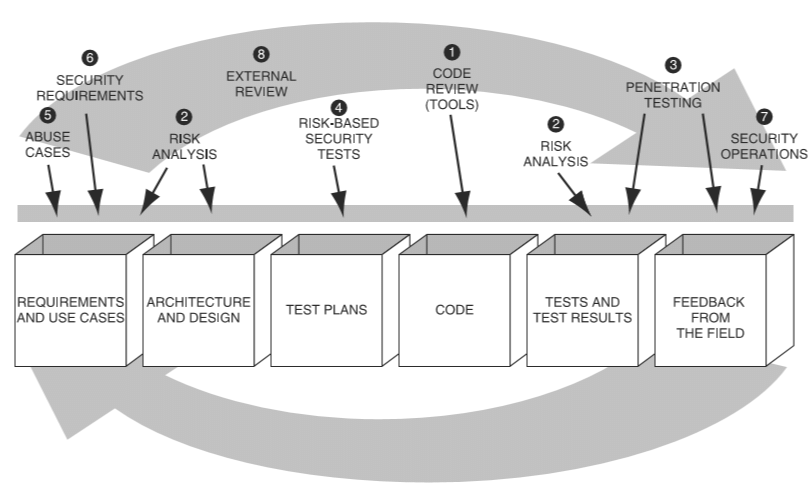
\includegraphics[width=0.5\linewidth]{images/McGraws-Secure-Software-Development-Life-Cycle-Process.png}
    \caption{McGraw's Secure Software Development Lifecycle (SSDLC) emphasizes integrating security at various stages of software development.}
    \end{center}
\end{figure}
\end{document}
